% (The MIT License)
%
% Copyright (c) 2023 Yegor Bugayenko
%
% Permission is hereby granted, free of charge, to any person obtaining a copy
% of this software and associated documentation files (the 'Software'), to deal
% in the Software without restriction, including without limitation the rights
% to use, copy, modify, merge, publish, distribute, sublicense, and/or sell
% copies of the Software, and to permit persons to whom the Software is
% furnished to do so, subject to the following conditions:
%
% The above copyright notice and this permission notice shall be included in all
% copies or substantial portions of the Software.
%
% THE SOFTWARE IS PROVIDED 'AS IS', WITHOUT WARRANTY OF ANY KIND, EXPRESS OR
% IMPLIED, INCLUDING BUT NOT LIMITED TO THE WARRANTIES OF MERCHANTABILITY,
% FITNESS FOR A PARTICULAR PURPOSE AND NONINFRINGEMENT. IN NO EVENT SHALL THE
% AUTHORS OR COPYRIGHT HOLDERS BE LIABLE FOR ANY CLAIM, DAMAGES OR OTHER
% LIABILITY, WHETHER IN AN ACTION OF CONTRACT, TORT OR OTHERWISE, ARISING FROM,
% OUT OF OR IN CONNECTION WITH THE SOFTWARE OR THE USE OR OTHER DEALINGS IN THE
% SOFTWARE.

\documentclass{article}
\usepackage[template,scheme=light,nominutes]{ppt-slides}
\usepackage{clicks}
\usepackage{../../lecture-notes/notes}
\usepackage{svg}
\usepackage{tikz}
  \usetikzlibrary{shadows}

\graphicspath{{../../faces/}}

\newcommand*{\thetitle}{Coders vs. Researchers}
\newcommand*{\thesubtitle}{How to be both?}
\newcommand*{\theauthor}{Yegor Bugayenko}

\begin{document}

\pptLeft{%
  \includesvg[height=2em]{../../lecture-notes/logos/innopolis.svg}\\
  November 23th, 2024}
\pptRight{@yegor256}

\definecolor{innoBackground}{HTML}{16240E}
\pagecolor{innoBackground}
\plush{
  \begin{pptMiddle}
    \includesvg[height=4em]{logo.svg}
    \pptTitle{\thetitle}{\thesubtitle}\par
    {\color{white}\scshape \theauthor}
    \newline
    {\color{white}\small Zerocracy\par}
  \end{pptMiddle}
}
\newpage
\pagecolor{white}

\print{
  \begin{textblock}{13}(2,11)%
    \tiny
    \(^\text{1}\) \url{https://www.statista.com/statistics/627312/}\\
    \(^\text{2}\) \url{https://github.blog/news-insights/company-news/100-million-developers-and-counting/}\\
    \(^\text{3}\) \url{https://uis.unesco.org/sites/default/files/documents/unesco-science-report-towards-2030-part1.pdf}\\
    \(^\text{4}\) \url{https://en.wikipedia.org/wiki/Software_engineering_demographics}\\
    \(^\text{5}\) \url{https://stackexchange.com/sites}\\
  \end{textblock}%
}
\plick{
  \begin{textblock}{4}(5,3)%
    How many \textcolor{orange}{programmers} are out there in the world?
  \end{textblock}%
}
\plick{
  \begin{textblock}{4}(5,6)%
    {\Huge 28.7M\(^\text{\scriptsize 1}\)}\par
    100M GitHub accounts\(^\text{2}\)\par
    27M StackOverflow users\(^\text{5}\)\par
  \end{textblock}%
}
\plick{
  \begin{textblock}{4}(10,3)%
    How many computer science \textcolor{orange}{researchers}?
  \end{textblock}%
}
\plush{
  \begin{textblock}{4}(10,6)%
    {\Huge 4M\(^\text{\scriptsize 3, 4}\)}\par
  \end{textblock}%
}

\lnThought*{What exactly is R\&D?}

\lnQuote
  [Richard Nelson]
  {richard-nelson}
  {Scientific \textcolor{orange}{research} may be defined as the human activity directed toward the advancement of knowledge, where knowledge is of two roughly separable sorts: \begin{inparaenum}[1)]\item \ul{facts or data} observed in reproducible experiments and
  \item \ul{theories or relationships} between data\end{inparaenum}.}
  {nelson1959simple}

\lnThought*{While research discovers laws of nature, development exploits them.}

\plick{
  \begin{textblock}{4}(1,3)%
    Imagine a task for Rust \textcolor{orange}{developer}: ``Implement a lookup function, capable of finding user IDs by their names.''\par
    {\ttfamily\scriptsize
    use std::collections::HashMap;\\
    ~\\
    let mut map: Map<String, i16> = \\
    ~~HashMap::new();\\
    ~\\
    map.insert("Jeff".to_string(), 42);\\
    map.insert("Lucie".to_string(), 17);\\
    // +N more items here\\
    ~\\
    let id = map.get("Jeff");
    }
  \end{textblock}%
}
\plick{
  \begin{textblock}{4}(6,3)%
    \textcolor{orange}{RQ}: ``Whether HashMap is the best possible map implementation for \(N < 20\)?''\par
    Answer:\par
    \raisebox{-9em}{\begin{tikzpicture}
    \scope[transform canvas={rotate=-3}]
    \node[draw=gray,drop shadow,fill=white,anchor=south west] {
      \parbox{.8\linewidth}{
        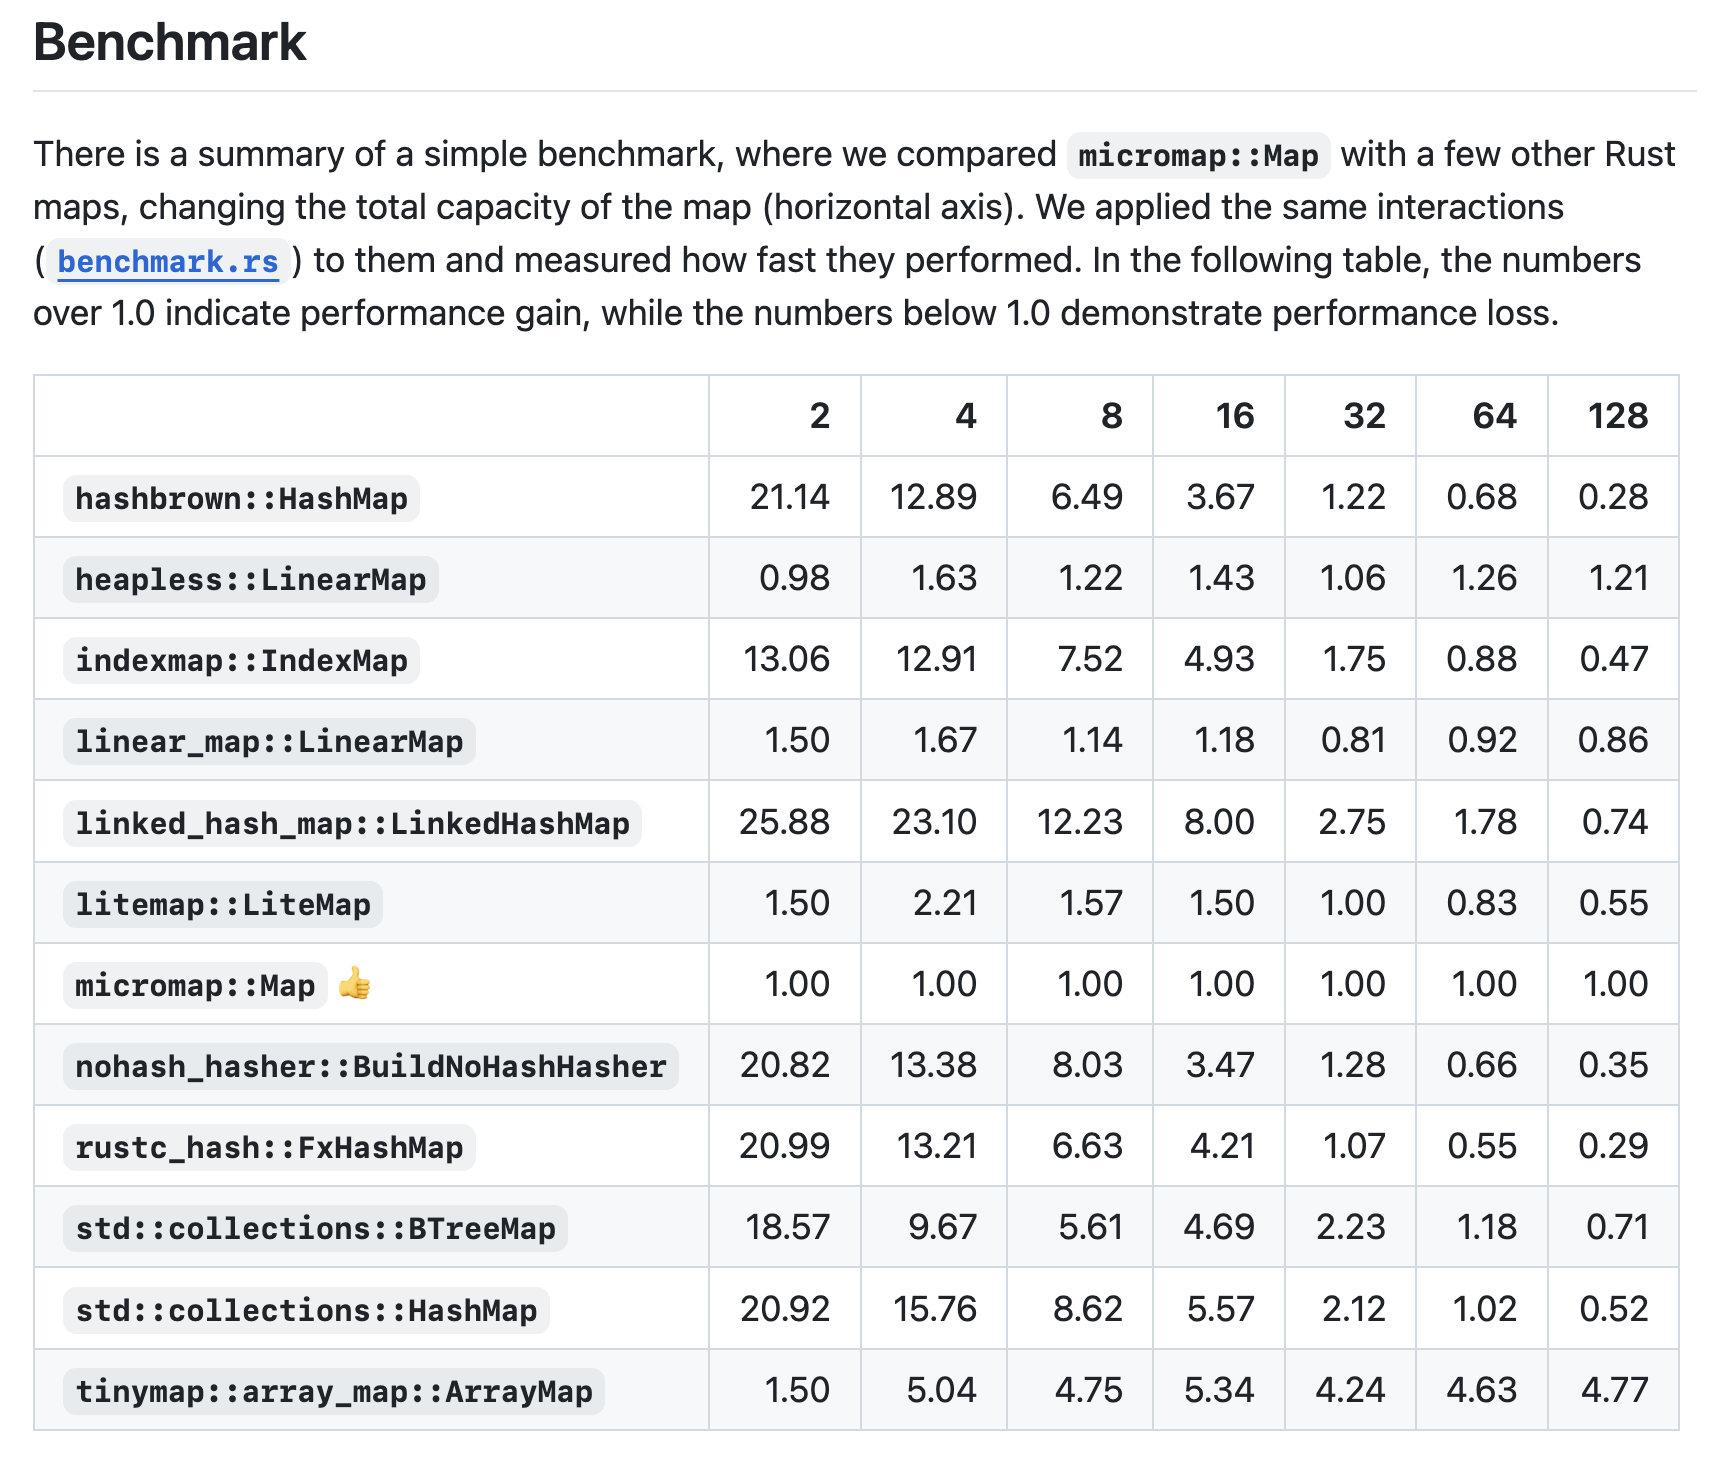
\includegraphics[width=\linewidth]{../2024-10-neimark/benchmark.png}\\
        {\tiny\url{https://github.com/yegor256/micromap}\par}
      }
    };
    \endscope
    \end{tikzpicture}}
  \end{textblock}%
}
\plush{
  \begin{textblock}{4}(11,3)%
    New \textcolor{orange}{implementation}, based on the \textcolor{orange}{law of nature} just discovered:\par
    {\ttfamily\scriptsize
    use std::collections::HashMap;\\
    ~\\
    \textcolor{orange}{if (N > 20)} \{ \\
    ~~map = HashMap::new();\\
    \} else \{\\
    ~~map = \textcolor{orange}{micromap::Map::new()};\\
    \}\\
    }
  \end{textblock}%
}
\flush{}

\lnThought*{How much \ul{criteria of success} is different for researchers and developers?}

\plush{
  \begin{multicols}{2}
  \pptBanner{Happy users:}\par
  \pptPic{.7}{customers.jpg}
  \par\columnbreak\par
  \pptBanner{Impressed reviewers:}\par
  \pptPic{.7}{reviewers.jpg}
  \end{multicols}
  {\tiny The images were generated by Kandinsky Telegram bot: \url{https://t.me/kandinsky21_bot}\par}}

\lnThought*{What's in it for me?}

\lnQuote
  [Aristotle]
  {aristotle}
  {Since happiness is a \ul{working} in the way of excellence, the man of science will be most happy.}
  {aristotle1897nicomachean}

\plush{
  \pptBanner{ChatGPT o1 Team:}
  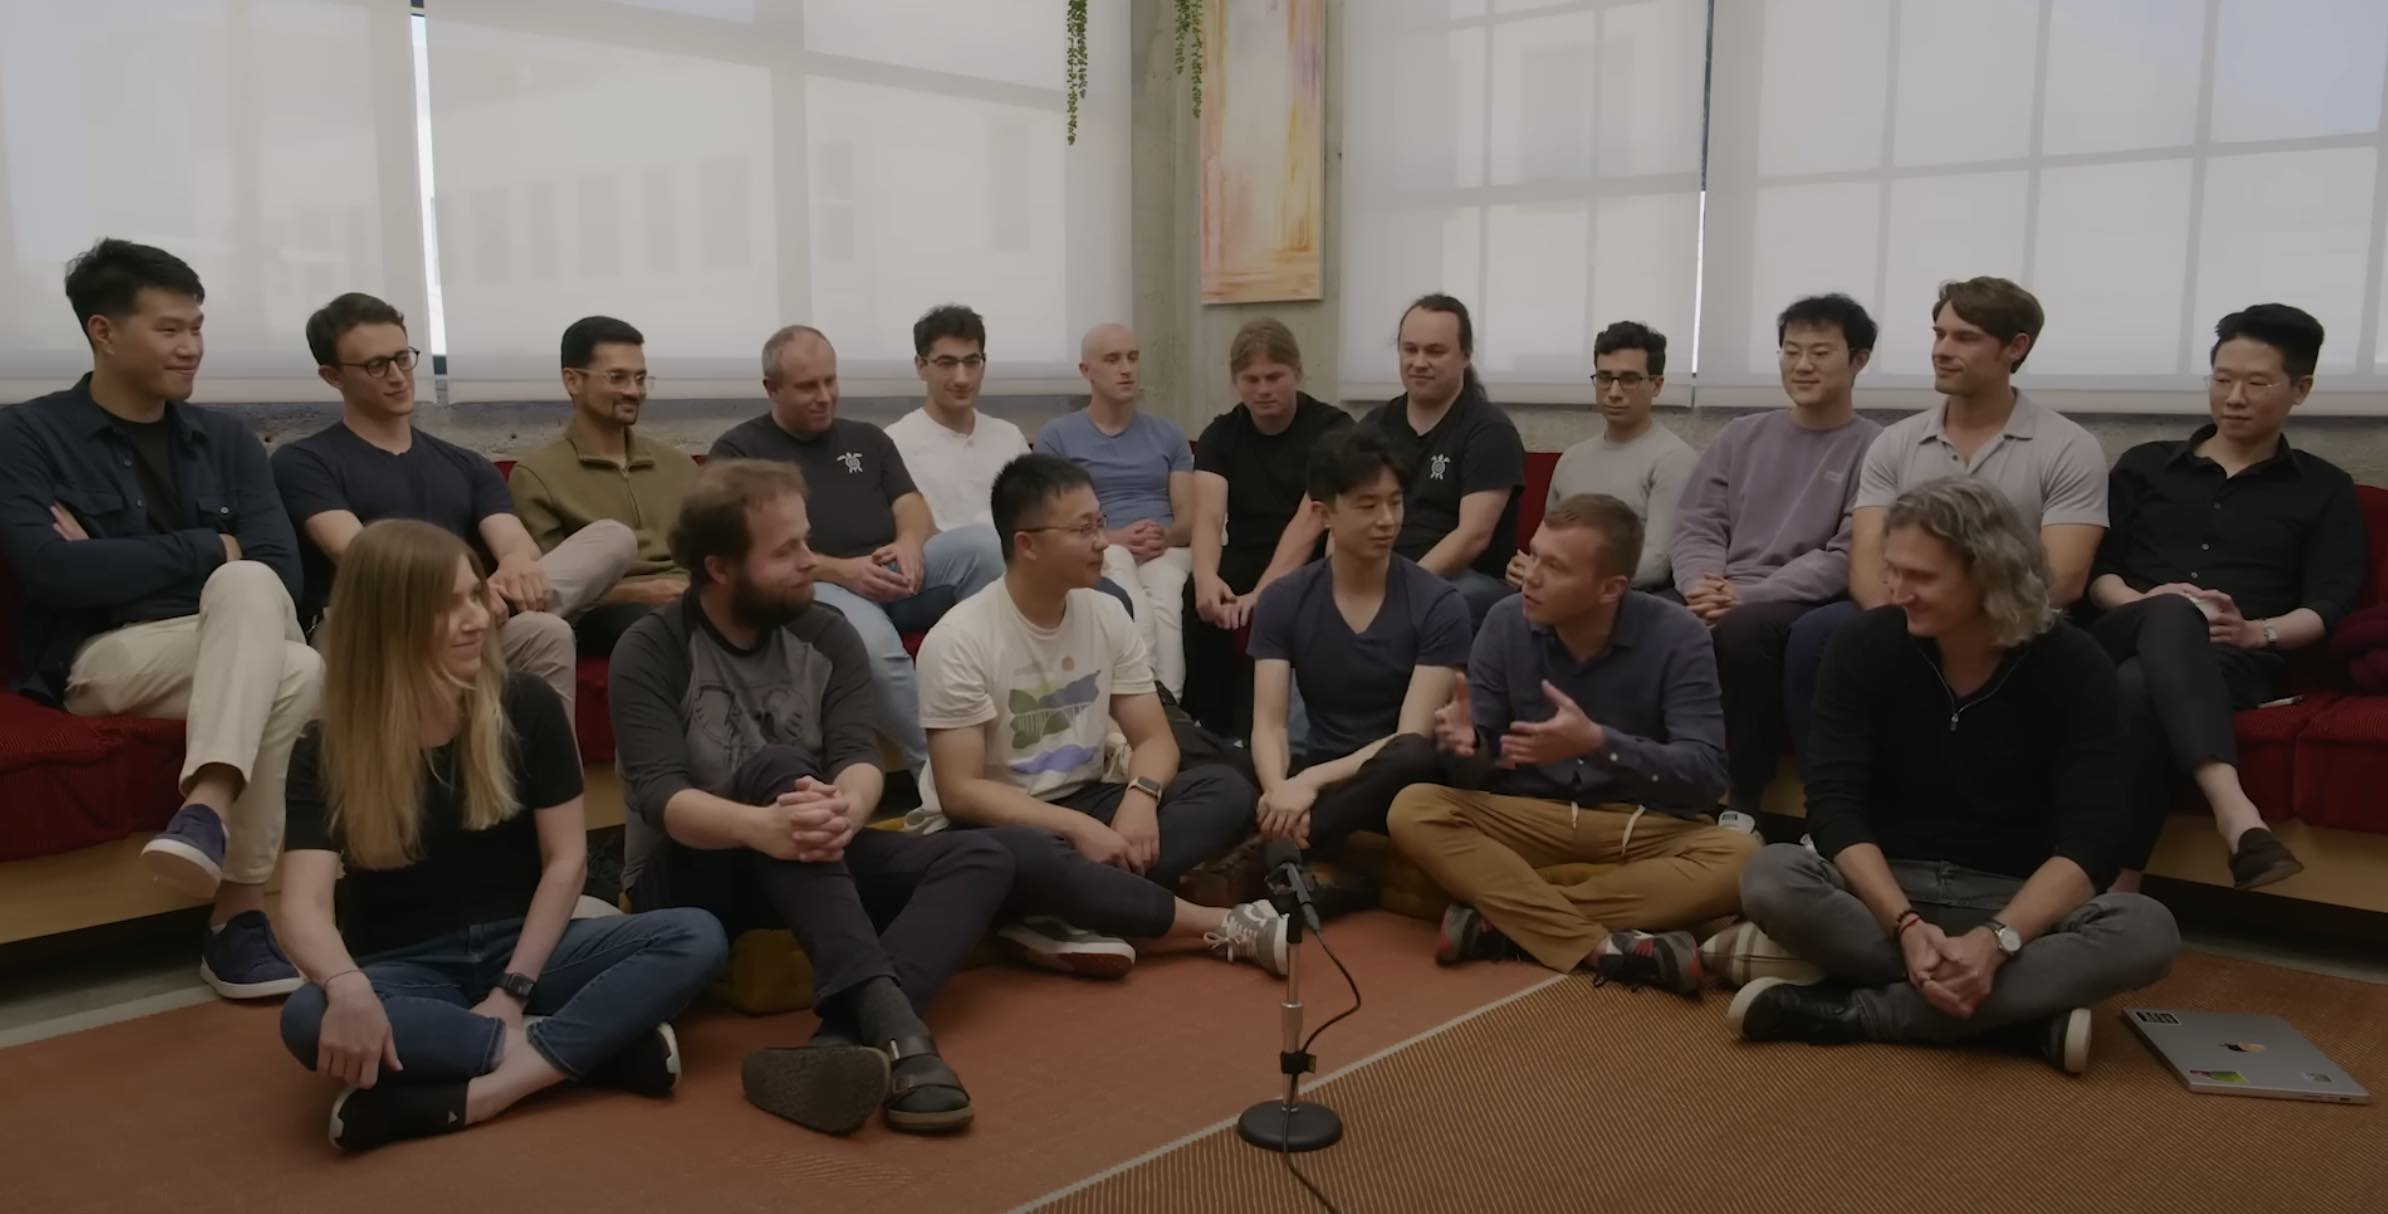
\includegraphics[width=.8\linewidth]{openai-before.jpg}\par
  {\small20-Sep-24: \url{https://www.youtube.com/watch?v=tEzs3VHyBDM}\par}}

\plush{
  \pptBanner{ChatGPT o1 Team:}
  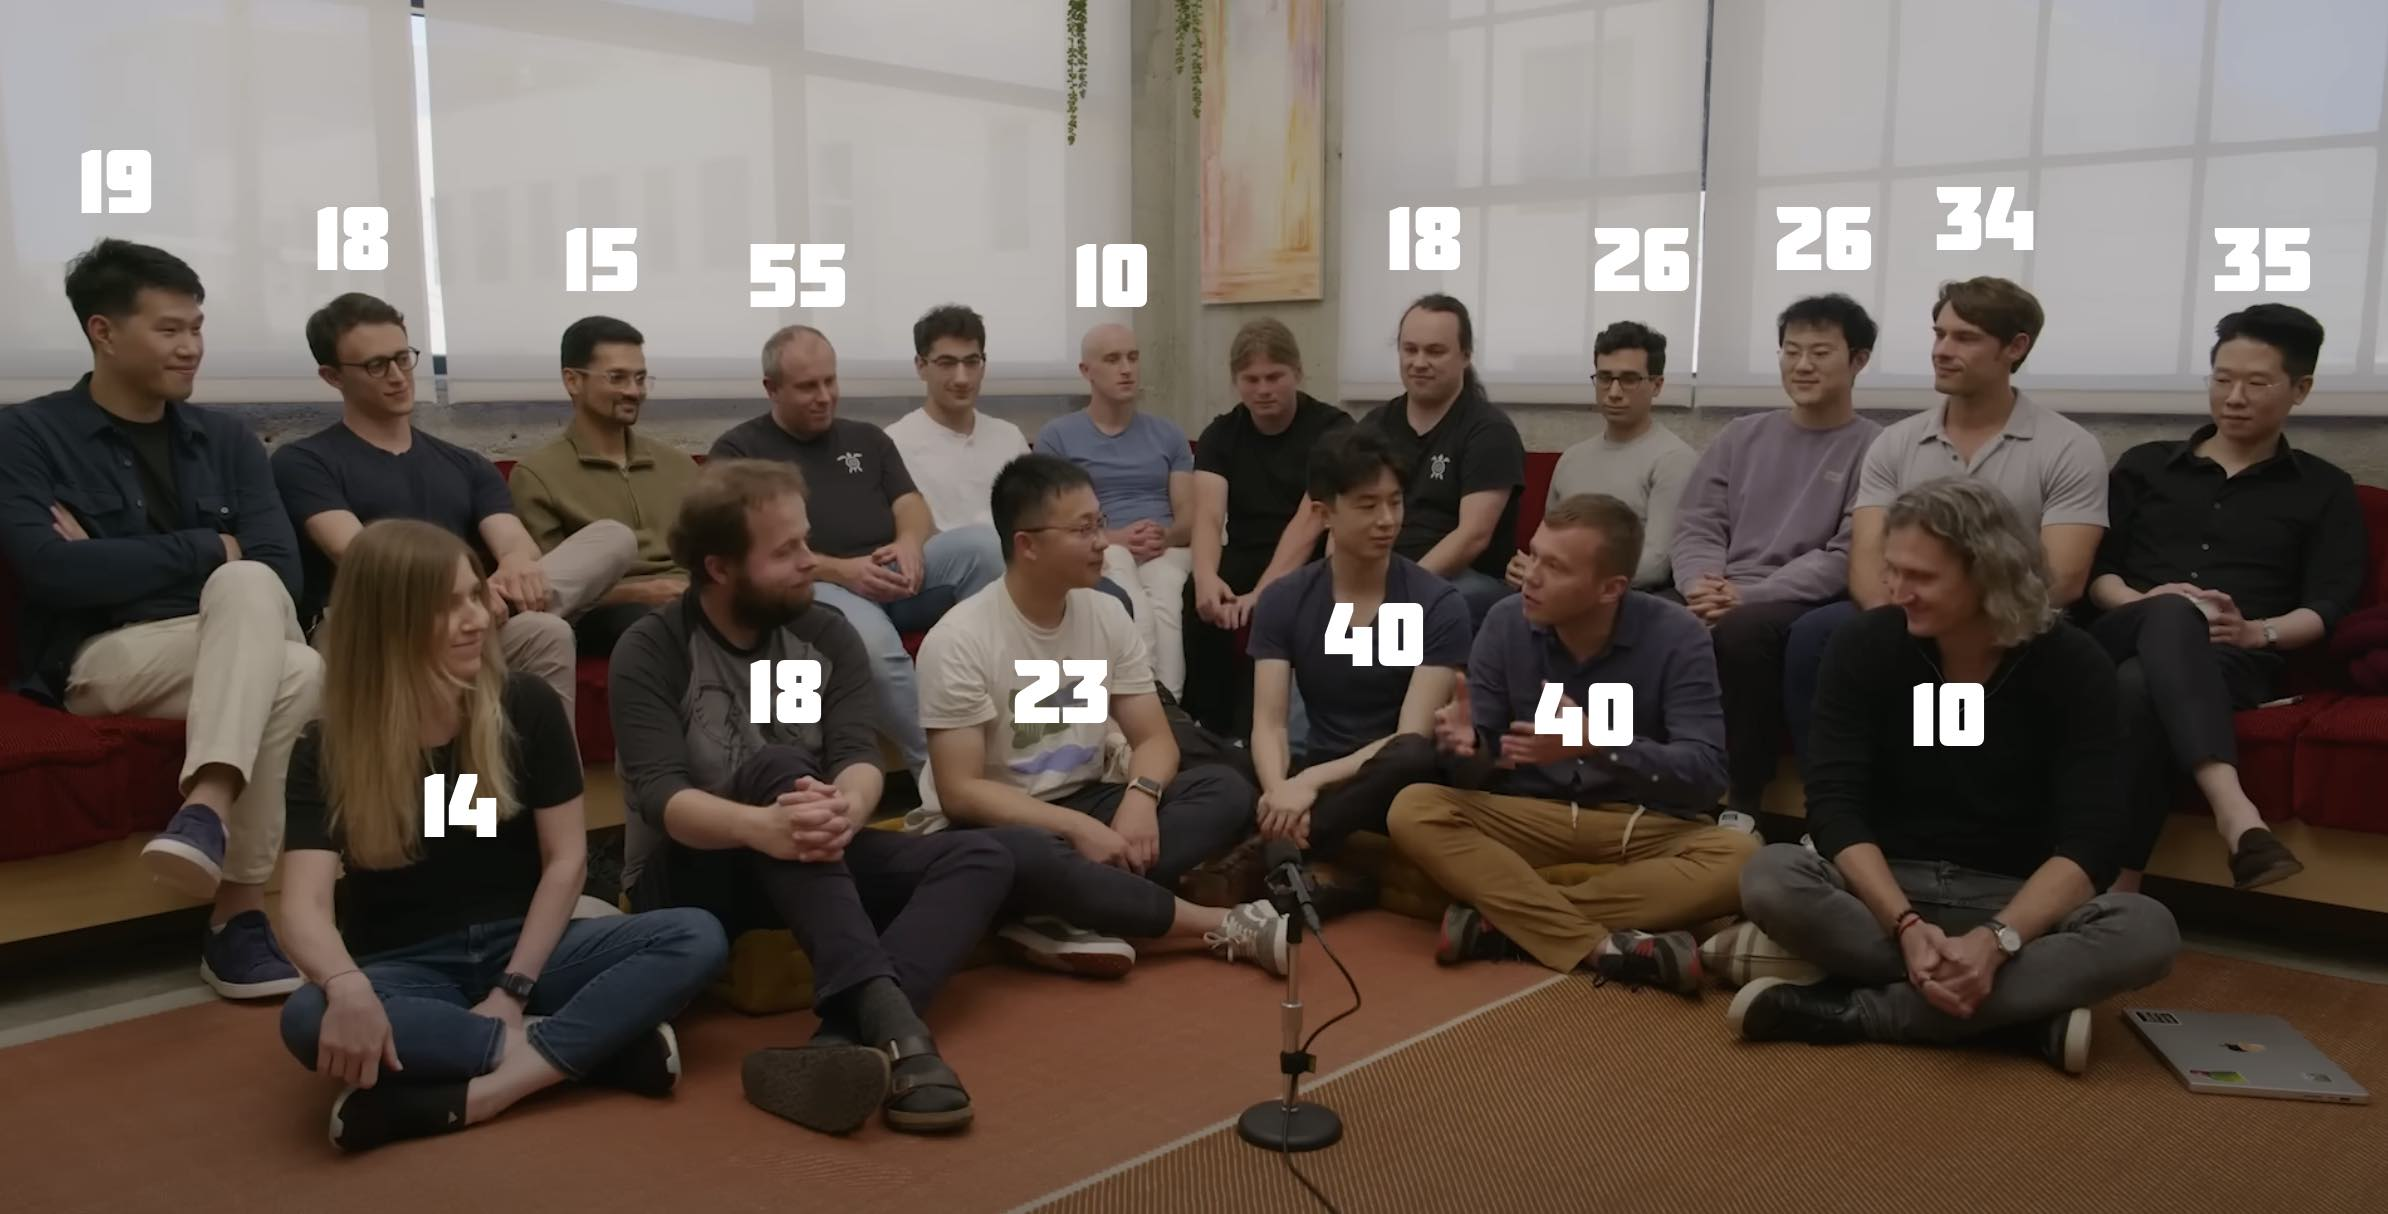
\includegraphics[width=.8\linewidth]{openai-after.jpg}\par
  {\small20-Sep-24: \url{https://www.youtube.com/watch?v=tEzs3VHyBDM}\par}}

\plush{
  \pptBanner{What is an Article Worth?}
  \begin{multicols}{2}
  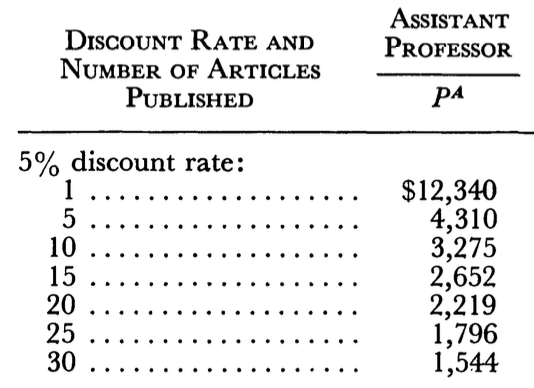
\includegraphics[width=\linewidth]{worth.png}
  \par\columnbreak\par
  ``The lifetime return to publication of the first article for an assistant professor is \textcolor{gray}{\st{\$12,340}} \textcolor{orange}{\textbf{\$71,928} (in 2024)}. The returns to additional publication diminish rapidly at first but at a lesser rate as the number of publications continues to increase.''
  \lnSource{tuckman1975article}
  \end{multicols}}

\lnQuote
  [Jo{\~a}o Ricardo Faria]
  {joao-ricardo-faria}
  {Using data from three separate state university systems, each comprised of research-focused institutions, we find that the marginal impact of an \ul{additional academic publication} on a scholar's citations increases that scholar’s pay by anywhere \textcolor{orange}{from 2.8 to 8.9\%}.}
  {faria2021marginal}

\plush{
  \pptBanner{What is a Citation Worth?}
  \begin{multicols}{2}
  \raisebox{-13em}{\begin{tikzpicture}
    \scope[transform canvas={rotate=-3}]
    \node[draw=gray,drop shadow,fill=white,anchor=south west] {
      \parbox{.6\linewidth}{
        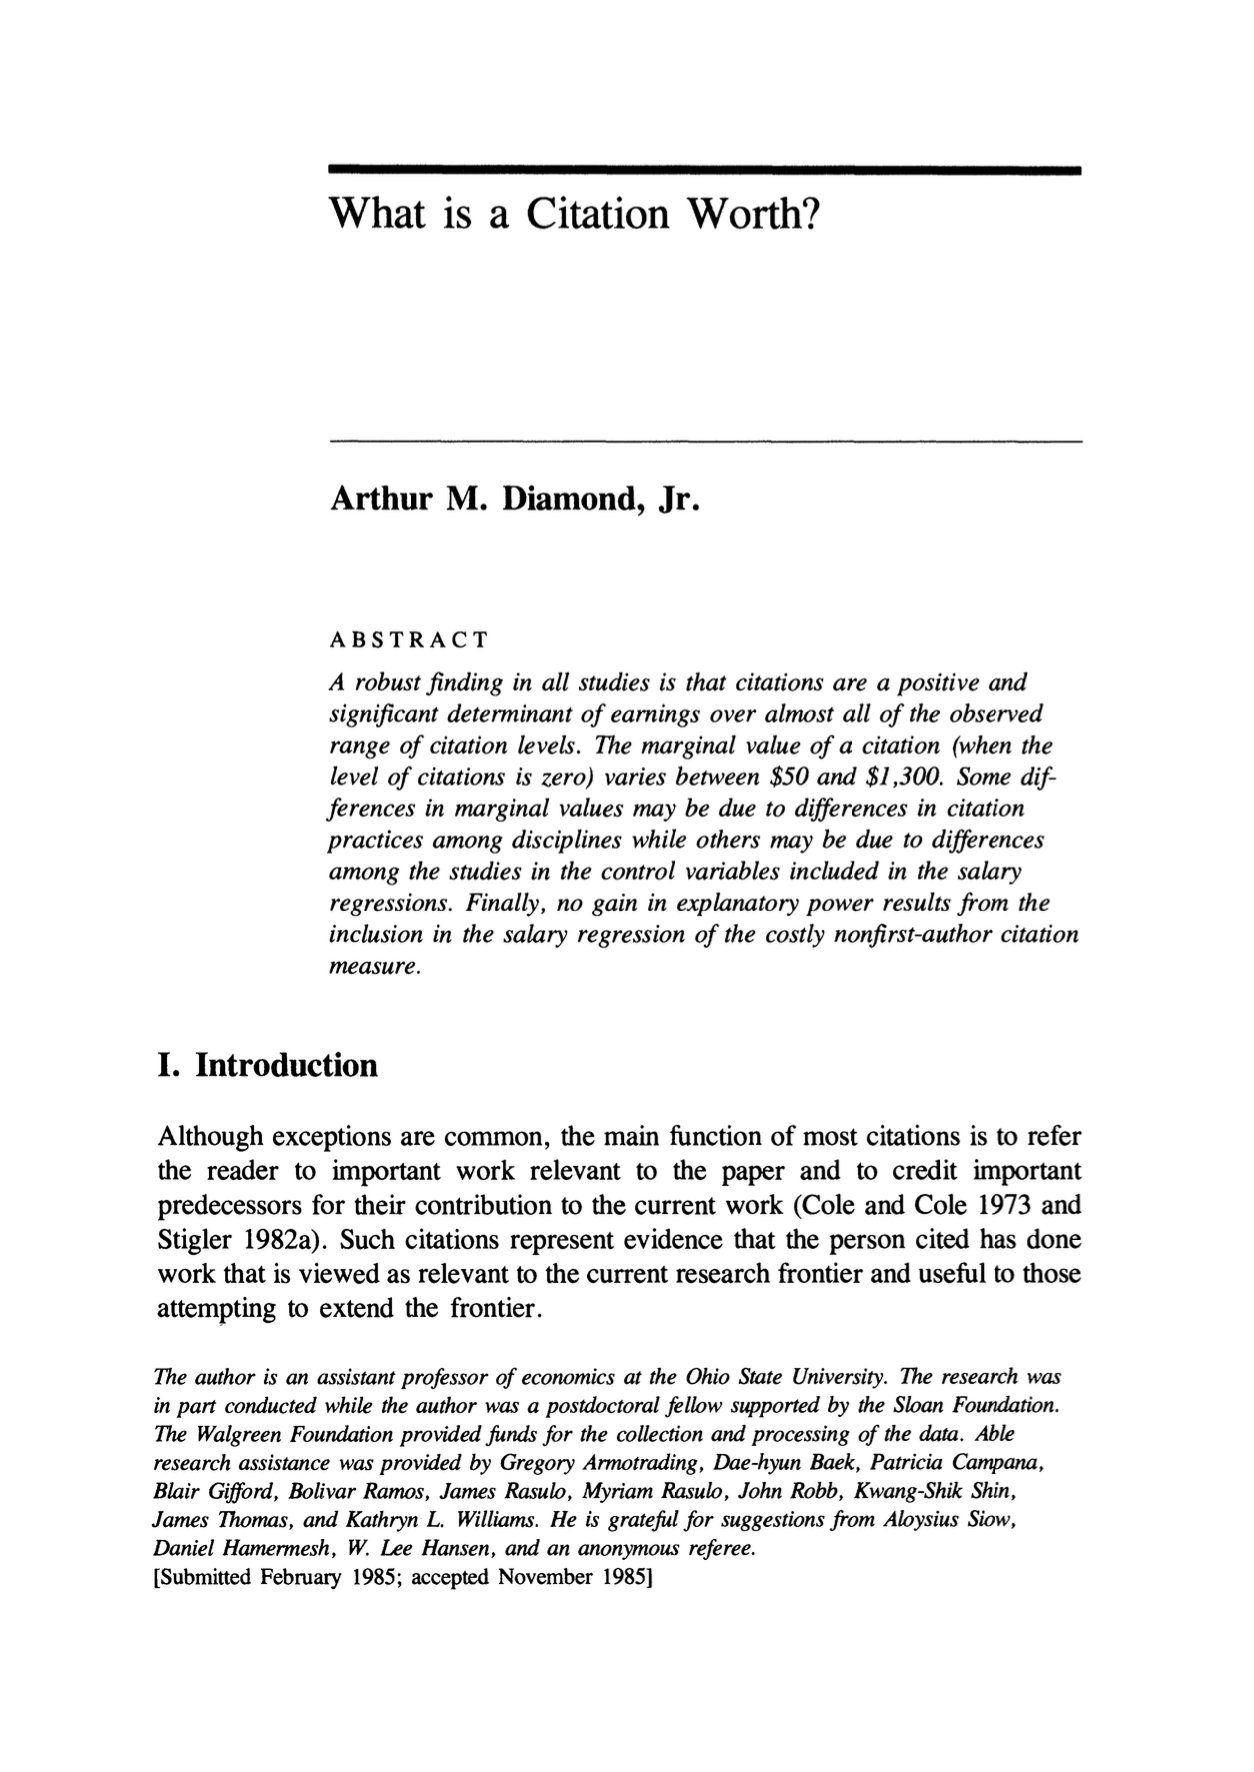
\includegraphics[width=\linewidth]{citation-worth.png}
      }
    };
    \endscope
    \end{tikzpicture}
  }
  \par\columnbreak\par
  ``At a level of zero citations, the marginal value of a citation to a nonfirst-author article is \textcolor{gray}{\st{\$314}} \textcolor{orange}{\$899}, while that of a citation to a first-author source is \textcolor{gray}{\st{\$402}} \textcolor{orange}{\$1,150}.''
  \lnSource{diamond1986citation}
  \end{multicols}}

\plush{
  \pptBanner{Is It Worth Getting a PhD?}
  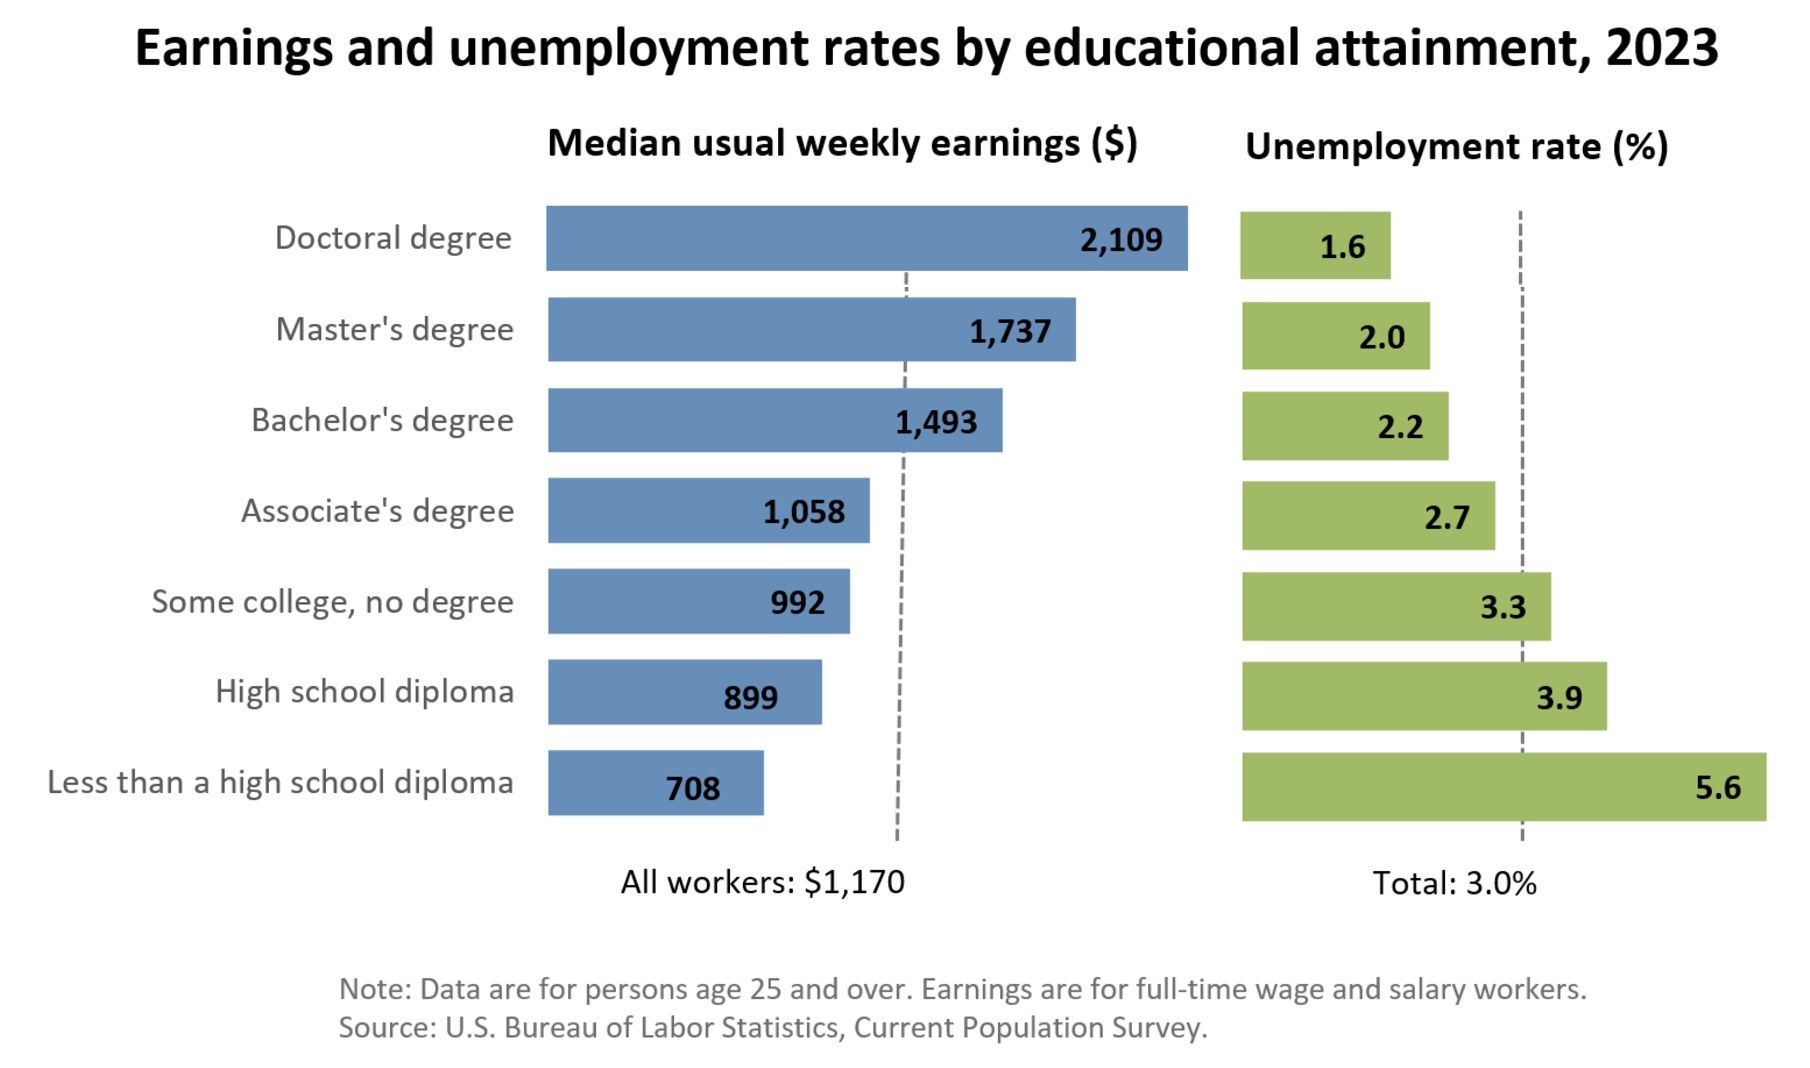
\includegraphics[width=.7\linewidth]{bureau.jpg}\par
  {\scriptsize\url{https://www.bls.gov/emp/chart-unemployment-earnings-education.htm}\par}}

\lnThought*{How about a few more examples of RQs?}

\lnPitch{
  \pptBanner[orange]{RQ1: How long Java objects live after instantiation?}
  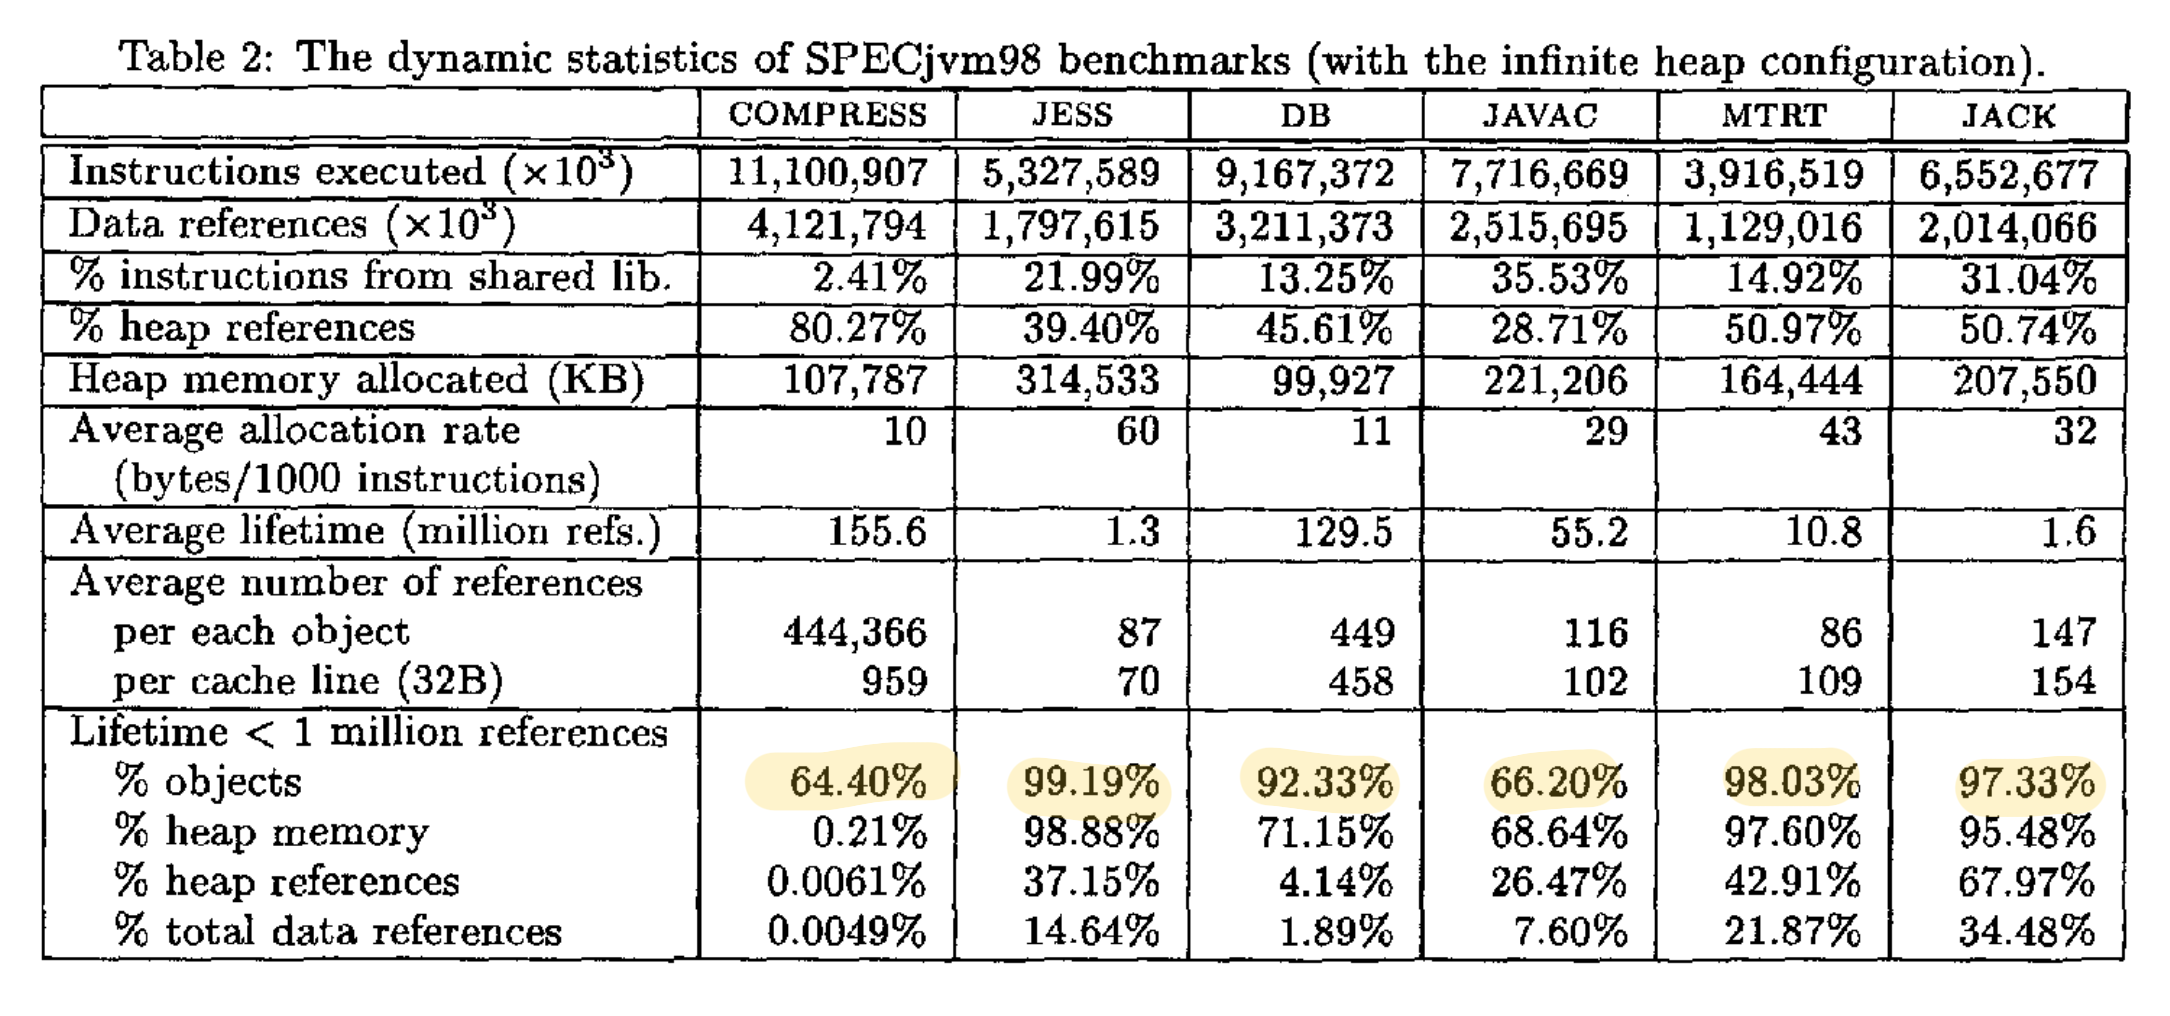
\includegraphics[width=.6\linewidth]{spec.png}
  \par
  ``We observe that Java programs generate a substantial amount of \ul{short-lived objects} (up to 99\%).''
  \lnSource{kim2000memory}}

\print{\pptBanner[orange]{RQ2: Larger pull requests mean lower quality?}}
\lnQuote
  [\nospell{Caitlin Sadowski}]
  {caitlin-sadowski}
  {A correlation between \ul{change size} and \ul{review quality} is acknowledged by Google and developers are strongly encouraged to make small, incremental changes (with the exception of large deletions and automated refactoring).}
  {sadowski2018modern}

\plush{
  \pptBanner[orange]{RQ3: Blank lines inside Java methods are code smell?}
  \begin{multicols}{2}
  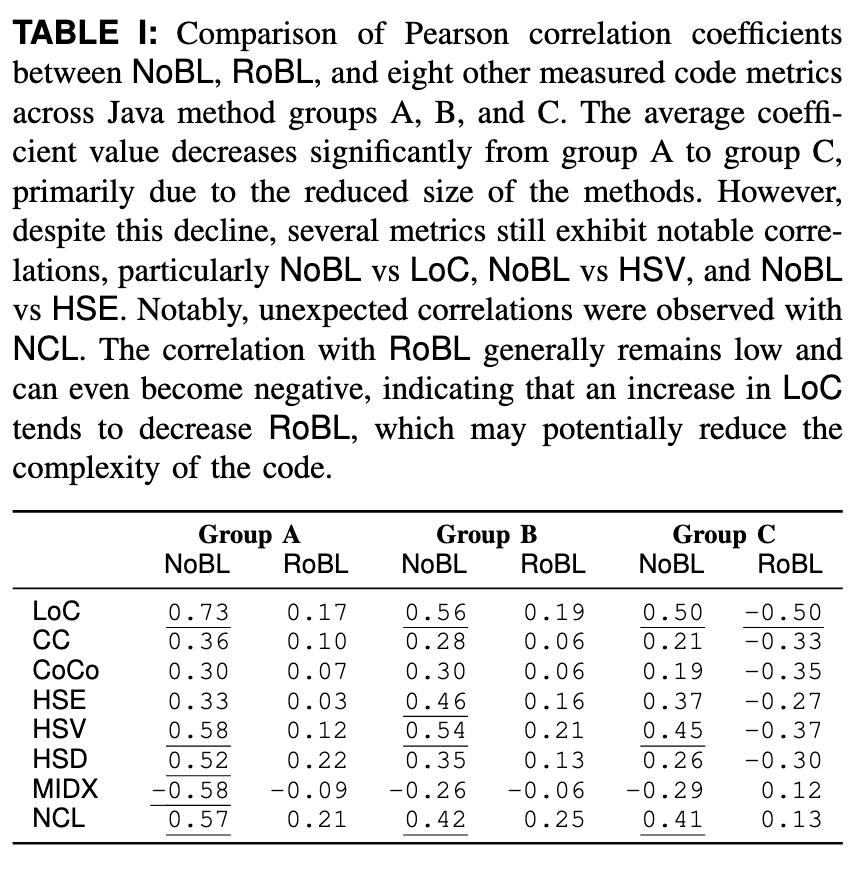
\includegraphics[width=.9\linewidth]{blank-lines.png}
  \par\columnbreak\par
  ``We analyzed 605,966 Java methods from 109 public repositories and
  found a moderate correlation between NoBL
  and complexity metrics such as LoC, HSV, HSE, and NCL,
  along with a positive non-linear relationship with MIDX.''
  \lnSource{galiullin2024}
  \end{multicols}}

\lnThought*{How to write and publish the first paper?}

\plick{\pptBanner{How to publish the first paper:}}
\plick{1) Read the book \textit{Write for Computer Science} by \citet{zobel2004writing}.}
\plick{2) Read the book about \LaTeX{} by \citet{lamport1994latex}.}
\plick{3) Subscribe, for example, to the \textbf{SEWorld} mailing list.}
\plick{4) Find a venue at \href{https://github.com/yegor256/awesome-cfp}{yegor256/awesome-cfp}.}
\plick{5) Find a professor to supervise your writing.}
\plick{6) Write it up, using the \href{https://www.yegor256.com/2024/02/06/research-flow.html}{Research Flow} process.}
\plush{7) Submit and wait for 2--3 months.}

\lnThought*{How to convince an employer that research matters?}

\lnQuote
  [Kenneth Joseph Arrow]
  {kenneth-joseph-arrow}
  {We expect a free enterprise economy to \textcolor{orange}{underinvest} in invention and research (as compared with an \ul{ideal}) because it is risky, because the product can be appropriated only to a limited extent, and because of increasing returns in use. This underinvestment will be greater for more \ul{basic} research.}
  {arrow1972economic}

\lnQuote
  [Bronwyn Hall]
  {bronwyn-hall}
  {First and most importantly, in practice \textcolor{orange}{50\% or more} of R\&D spending is the \ul{wages and salaries} of highly educated \ul{scientists and engineers}. Their efforts create an intangible asset, the firm’s knowledge base, from which profits in future years will be generated. To the extent that this knowledge is `tacit' rather than codified, it is embedded in the human capital of the firm's employees, and is therefore lost if they \ul{leave} or are \ul{fired}.}
  {hall2002financing}

\plick{\pptBanner{What can we do?}}
  \plick{Option 1: Change the employer}
  \plush{Option 2: Don't tell them}

\lnThought*{What's next?}

\plush{
  \begin{multicols}{2}
  \pptBanner{1)~Subscribe:}\par
  \qrcode[height=8em]{https://t.me/yegor256news}\par
  \href{https://t.me/yegor256news}{\texttt{@yegor256news}}
  \par\columnbreak\par
  \pptBanner{2)~Join:}\par
  Text me in Telegram, to join one of our research projects (instead of inventing your own):\par
  {\Huge\texttt{@yegor256}}
  \end{multicols}}

\end{document}
